%Authors guidlines: http://royalsocietypublishing.org/instructions-authors
% 2500 words max (includes the title page, abstract, references, acknowledgements and figure/table legends)
% current version is around 3700. I think a big cut down can be done on the references.
% We allow a maximum of 4 displays, only 2 of which can be figures.

\documentclass[12pt,letterpaper]{article}
\usepackage{natbib}

%Packages
\usepackage{pdflscape}
\usepackage{fixltx2e}
\usepackage{textcomp}
\usepackage{fullpage}
\usepackage{float}
\usepackage{latexsym}
\usepackage{url}
\usepackage{epsfig}
\usepackage{graphicx}
\usepackage{amssymb}
\usepackage{amsmath}
\usepackage{bm}
\usepackage{array}
\usepackage[version=3]{mhchem}
\usepackage{ifthen}
\usepackage{caption}
\usepackage{hyperref}
\usepackage{amsthm}
\usepackage{amstext}
\usepackage{enumerate}
\usepackage[osf]{mathpazo}
\usepackage{dcolumn}
\usepackage{lineno}
\usepackage{longtable}
\pagenumbering{arabic}

\newcolumntype{L}[1]{>{\raggedright\let\newline\\\arraybackslash\hspace{0pt}}m{#1}}
\newcolumntype{C}[1]{>{\centering\let\newline\\\arraybackslash\hspace{0pt}}m{#1}}
\newcolumntype{R}[1]{>{\raggedleft\let\newline\\\arraybackslash\hspace{0pt}}m{#1}}

%Pagination style and stuff % NC: Note that these are all syst biol specific.
\linespread{2}
\raggedright
\setlength{\parindent}{0.5in}
\setcounter{secnumdepth}{0} 
\renewcommand{\section}[1]{%
\bigskip
\begin{center}
\begin{Large}
\normalfont\scshape #1
\medskip
\end{Large}
\end{center}}
\renewcommand{\subsection}[1]{%
\bigskip
\begin{center}
\begin{large}
\normalfont\itshape #1
\end{large}
\end{center}}
\renewcommand{\subsubsection}[1]{%
\vspace{2ex}
\noindent
\textit{#1.}---}
\renewcommand{\tableofcontents}{}
%\bibpunct{(}{)}{;}{a}{}{,}

%---------------------------------------------
%
%       START
%
%---------------------------------------------

\begin{document}

%Running head
\begin{flushright}
Version dated: \today
\end{flushright}
\bigskip
\noindent RH: Morphological data availability in living mammals

\bigskip
\medskip
\begin{center}

\noindent{\Large \bf Morphological data is lacking for living mammals}
%Or: Missing cladistic data in living mammals - but I prefer the first one emphasizing on the availability of it. The data is not missing per se, it's just not coded!
% NC: sometimes the better title is one that answers the question rather than giving the topic. e.g., "Morphological data is lacking for living species" or similar
% TG: maybe worth considering the special issue as well? "Putting fossils in tree" so maybe something like "There is not enough morphological data for living mammals to branch fossils in the trees."
% TG: or some poetic... "Living and dead mammals: morphological data is lacking in living for combined analysis"
\bigskip

\noindent {\normalsize \sc Thomas Guillerme$^1$$^,$$^2$$^,$$^*$ and Natalie Cooper$^1$$^,$$^2$$^,$$^3$}\\
\noindent {\small \it 
$^1$School of Natural Sciences, Trinity College Dublin, Dublin 2, Ireland.\\
$^2$Trinity Centre for Biodiversity Research, Trinity College Dublin, Dublin 2, Ireland.\\ %Should we remove that one for word count?
$^3$Department of Life Sciences, Natural History Museum, Cromwell Road, London, SW7 5BD, UK.}\\
\end{center}
\medskip
\noindent{*\bf Corresponding author.} \textit{Zoology Building, Trinity College Dublin, Dublin 2, Ireland; E-mail: guillert@tcd.ie; Fax: +353 1 6778094; Tel: +353 1 896 2571.}\\  
\vspace{1in}

%Line numbering
\modulolinenumbers[1]
\linenumbers

%---------------------------------------------
%
%       ABSTRACT
%
%---------------------------------------------
% NC: Time to sort this out!
\newpage
\begin{abstract} % 200 words, all keywords written in abstract if possible. TG: That's 195 words for now.
Combining living and fossil in the same analysis data is crucial for studying changes in global biodiversity through time.
One method allowing to combine this data is the Total Evidence method that uses both molecular data for living species and morphological data for both living and fossil species.
With this method, a good overlap of morphological data between living and fossil taxa is crucial for accurately inferring the phylogenies’ topology.

Since the advent of DNA, molecular data has become easily and widely available.
However, despite two centuries of morphological studies, scientists using and generating such data mainly focus on palaeontological data.
Therefore, there is a gap in our knowledge of neontological morphological data even in well studied groups such as mammals.

In this study, we quantify the morphological data available for living mammal taxa.
We then analyse the structure of the available data by testing if it is clustered or evenly spread across the phylogeny.
We found that 78\% of mammalian orders have less than 25\% data available at the species level.
However, we found that the available is often randomly distributed among these orders apart from six of them where the data is clustered
\end{abstract}

%\noindent Key words: Total Evidence method, data structure, phylogenetic, fossil, topology\\ Excluded from word count.

\vspace{1.5in}

%---------------------------------------------
%
%       INTRODUCTION
%
%---------------------------------------------
\newpage 
\section{Introduction}
There is an increasing consensus among evolutionary biologists that studying both living and fossil taxa is essential for fully understanding macroevolutionary patterns and processes \citep{jacksonwhat2006,quentaldiversity2010,dietlconservation2011,slaterunifying2013,fritzdiversity2013,Wood01032013}.
For example, including both living and fossil taxa in evolutionary studies can improve the accuracy of timing diversification events \citep[e.g.][]{ronquista2012}, our understanding of relationships among lineages \citep[e.g.][]{beckancient2014}, and our ability to infer biogeographical patterns through time \citep[e.g.][]{Meseguer01032015}.
To perform such analyses it is necessary to combine living and fossil taxa in phylogenetic trees.
One increasingly popular method, the Total Evidence method \citep{eernissetaxonomic1993,ronquista2012}, combines molecular data from living taxa and morphological data from both living and fossil taxa in a supermatrix \citep[e.g.][]{pyrondivergence2011,ronquista2012,schragocombining2013,slaterunifying2013,beckancient2014,Meseguer01032015}, producing a phylogeny with living and fossil taxa at the tips. 
These phylogenies can be dated using methods such as tip-dating \citep{ronquista2012,Drummond01082012,Wood01032013} and incorporated into macroevolutionary studies \citep[e.g.][]{ronquista2012,Wood01032013,slaterphylogenetic2013}.

A downside of the Total Evidence method is that it requires a lot of data.
One must collect molecular data for living taxa and morphological data for both living and fossil taxa; two types of data that require fairly different technical skills (e.g. molecular sequencing \textit{vs.} anatomical description).
Additionally, large chunks of this data can be difficult, or even impossible, to collect for every taxon present in the analysis.
For example, fossils very rarely have molecular data and incomplete fossil preservation (e.g. soft \textit{vs.} hard tissues) may restrict the amount of morphological data available \citep{sansomfossilization2013}.
Additionally, since the molecular phylogenetics revolution, it has become less common to collect morphological characters for living taxa when molecular data is available (e.g. in \cite{slaterphylogenetic2013}, only 13\% of the 169 living taxa have coded morphological data).
Unfortunately this missing data can lead to errors in phylogenetic inference; in fact, simulations show that the ability of the Total Evidence method to recover the correct phylogenetic topology decreases when there is a low overlap between morphological data in the living and fossil taxa \citep{GuillermeCooper}, regardless the overall amount of morphological data available for the fossils (or the amount of molecular data available for the living species).
The effect of missing data on topology is greatest when living taxa have few morphological data.
This is because (1) a fossil cannot branch in the correct clade if there is no overlapping morphological data in the clade; and (2) a fossil has a higher probability of branching within a clade with more morphological data available for living taxa, regardless of whether this is the correct clade or not \citep{GuillermeCooper}. 

The issues above highlight that it is crucial to have sufficient morphological data for living taxa in a clade before using a Total Evidence approach.
However, it is unclear how much morphological data for living taxa is actually available (i.e. already coded from museum specimens and deposited in phylogenetic matrices accessible online), and how this data is distributed across clades.
Intuitively, most people assume this kind of data has already been collected, but empirical data suggest otherwise (e.g. in \cite{ronquista2012,slaterphylogenetic2013,beckancient2014}).
To investigate this further, we assess the amount of available morphological data for living mammals to determine whether sufficient data exists to build reliable Total Evidence phylogenies in this group.
We collected cladistic data (i.e. discrete morphological characters used in phylogenetics) from 286 phylogenetic matrices available online and measured the proportion of cladistic data available for each mammalian order.
%Additionally, if the available data is randomly distributed across clades, the topological errors should be less extreme than if the data is biased towards particulars groups.
Additionally, because missing morphological data in living species can influence tree topology as described above, %NC: Might still need to fix this sentence. "Topological caveats above" was too unclear.
we determined whether the available cladistic data was phylogenetically overdispersed or clustered in the mammalian orders where data was missing. 
We find that available morphological data for living mammals is scarce but generally randomly distributed across phylogenies. 
We recommend that efforts be made to collect and share more cladistic data for living species to improve the accuracy of Total Evidence phylogenies.

% NC: If there are word count problems we can ditch the last two sentences.
%---------------------------------------------
%
%       METHODS
%
%---------------------------------------------
\section{Materials and Methods}
\subsection{Data collection and standardisation}
We downloaded all cladistic matrices containing any living and/or fossil mammal taxa from three major public databases (accessed 10th of June 2015): Morphobank \citep[\texttt{http://www.morphobank.org/};][]{morphobank}, Graeme Lloyd's website (\texttt{graemetlloyd.com/matrmamm.html}) and Ross Mounce's GitHub repository (\texttt{https://github.com/rossmounce/cladistic-data}).
We also performed a systematic Google Scholar search (accessed 11th of June 2015) for matrices that were not uploaded to these databases (see Supplementary Materials for a detailed description of the search procedure).
In total, we downloaded 286 matrices containing a total of 11010 operational taxonomic units (OTUs) of which 5228 were unique. % Number of unique OTUs (including fossils)
In this study, we refer to OTUs rather than species since the entries in the downloaded matrices were not standardised and ranged from specific individual specimen names (i.e. the name of a collection item) to the family-level.
Where possible, we considered OTUs at their lowest valid taxonomic level (i.e. species) but some OTUs were only valid at a higher taxonomic level (e.g. genus or family).
Therefore for some orders, we sampled more genera than species (Table \ref{Table_morpho_taxa_proportion}).

To select the lowest valid taxonomic level for each OTU, we standardised their taxonomy by correcting species names so they matched standard taxonomic nomenclature (e.g., \textit{H. sapiens} was transformed to \textit{Homo sapiens}).
We designated as ``living'' all OTUs that were either present in the phylogeny of \citet{BinindaEmonds} or the taxonomy of \citet{wilson2005mammal}, and designated as ``fossil'' all OTUs that were present in the Paleobiology database (\texttt{https://paleobiodb.org/}).
For OTUs that did not appear in these three sources, we first decomposed the name (i.e. \textit{Homo sapiens} became \textit{Homo} and \textit{sapiens}) and tried to match the first element with a higher taxonomic level (family, genus etc.).
Any OTUs that still had no matches in the sources above were designated as non-applicable (NA; see Supplementary Material for more details).

The number of characters in each matrix ranged from 6 to 4541.
Matrices with few characters are problematic when comparing available data among matrices because (1) they have less chance of having characters that overlap with those of other matrices \citep{wagner2000} and (2) they are more likely to contain a higher proportion of specific characters that are not-applicable across large clades \citep[][e.g. ``antler ramifications'' is a character that is only applicable to Cervidae not all mammals]{Brazeau2011}.
Therefore we selected only matrices containing \textgreater 100 characters for each OTU.
This threshold was chosen to correspond with the number of characters used in \citet{GuillermeCooper} and \citet{harrisonamong-character2014}.
Note that results of analyses with no character threshold are available in Supplementary Material. 
After removing all matrices with \textless 100 characters, we retained 1074 unique living mammal OTUs from 126 matrices for our analyses. % 1601 unique living OTUs for 286 matrices (no threshold)

\subsection{Data availability and distribution}
To assess the availability of cladistic data for each mammalian order, we calculated the percentage of OTUs with cladistic data at three different taxonomic levels: family, genus and species.
%We used these different taxonomic levels because some clades are well covered at the family- or genus-level, but poorly covered at the species-level. % NC: Probably obvious?
We consider orders with \textless 25\% of living taxa with cladistic data as having poor data coverage (``low'' coverage), and orders with \textgreater 75\% of living taxa with cladistic data as having good data coverage (hereafter ``high'' coverage). 

For orders with \textless 100\% cladistic data coverage at any taxonomic level, we investigated whether the available cladistic data was (i) randomly distributed, (ii) overdispersed or (iii) clustered, with respect to phylogeny, using two metrics from community phylogenetics: the Nearest Taxon Index \citep[NTI;][]{webb2002phylogenies} and the Net Relatedness Index \citep[NRI;][]{webb2002phylogenies}. 
NTI is most sensitive to clustering or overdispersion near the tips, whereas NRI is more sensitive to clustering or overdispersion across the whole phylogeny \citep{Cooper2008}. 
Both metrics were calculated using the \texttt{picante} package in R \citep{picante,R}.

NTI \citep{webb2002phylogenies} is based on mean nearest neighbour distance (MNND) and is calculated as follows:
  \begin{equation}
    NTI=-\left(\frac{\overline{MNND}_{obs}-\overline{MNND}_{n}}{\sigma(MNND_{n})}\right)
  \end{equation}
where $\overline{MNND}_{obs}$ is the observed mean distance between each of $n$ taxa with cladistic data and its nearest neighbour with cladistic data in the phylogeny, 
$\overline{MNND}_{n}$ is the mean of 1000 mean MNND between $n$ randomly drawn taxa, and $\sigma(MNND_{n})$ is the standard deviation of these 1000 random MNND values.
NRI is similar but is based on mean phylogenetic distance (MPD) as follows:
  \begin{equation}
    NRI=-\left(\frac{\overline{MPD}_{obs}-\overline{MPD}_{n}}{\sigma(MPD_{n})}\right)
  \end{equation}
where $\overline{MPD}_{obs}$ is the observed mean phylogenetic distance of the tree containing only the $n$ taxa with cladistic data, $\overline{MPD}_{n}$ is the expected random MPD for $n$ taxa estimated by calculating the MPD from $n$ taxa randomly drawn from the phylogeny and repeated 1000 times, and $\sigma(MPD_{n})$ is the standard deviation of the 1000 random MPD values. % NC: This can be shortened a bit but it's only gonna save you 50 words max.
Negative NTI and NRI values show that the focal taxa are more overdispersed across the phylogeny than expected by chance, and positive values reflect significant clustering.

We calculated NTI and NRI values for each mammalian order separately, at each different taxonomic level. 
For each analysis our focal taxa were those with available cladistic data at that taxonomic level and the phylogeny was the phylogeny of the order pruned from \citet{BinindaEmonds}.

%---------------------------------------------
%
%       RESULTS
%
%---------------------------------------------

\section{Results}
Across the 126 cladistic matrices we extracted, 22 out of 28 mammalian orders have low coverage (\textless 25\% of species with cladistic data) and six have high coverage (\textgreater 75\% of species with cladistic data) at the species-level.
At the genus-level, three orders have low coverage and 12 have high coverage, and at the family-level, no orders have low coverage and 23 have high coverage (Table \ref{Table_morpho_taxa_proportion}).

% latex table generated in R 3.2.0 by xtable 1.7-4 package
% Sat Jun 20 17:19:07 2015
\begin{longtable}{lL{1.8cm}C{2cm}lcc}
\caption{Number of taxa with available cladistic data for mammalian orders at three taxonomic levels (without any character threshold; results from the 286 matrices). The coverage represents the proportion of taxa with available morphological data. The left vertical bar represents 25\% of available data (``low'' coverage if \textless 25\%); The right vertical bar represents 75\% of available data (``high'' coverage if \textgreater 75\%). When the Net Relatedness Index (NRI) and the Nearest Taxon Index (NTI) are negative, taxa are more phylogenetically dispersed than expected by chance; when NRI or NTI are positive, taxa are more phylogenetically clustered by expected by chance. Significant NRI or NTI are highlighted in bold. *p \textless 0.05; **p \textless 0.01; ***p \textless 0.001.} \\ 
  \hline
Order & Taxonomic level & Proportion of taxa & Coverage & NRI & NTI \\ 
  \hline
Afrosoricida & family & 2/2 & 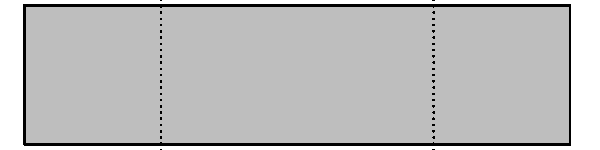
\includegraphics[width=0.20\linewidth, height=0.05\linewidth]{Table_figures/bar1.pdf} &   &   \\ 
  Afrosoricida & genus & 17/17 & 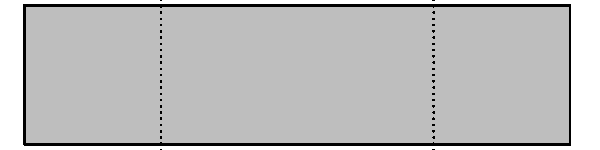
\includegraphics[width=0.20\linewidth, height=0.05\linewidth]{Table_figures/bar2.pdf} &   &   \\ 
  Afrosoricida & species & 23/42 & 
\includegraphics[width=0.20\linewidth, height=0.05\linewidth]{Table_figures/bar3.pdf} & 1.75 & 1.08 \\ 
  Carnivora & family & 14/15 & 
\includegraphics[width=0.20\linewidth, height=0.05\linewidth]{Table_figures/bar4.pdf} & 0.63 & 0.6 \\ 
  \textbf{Carnivora} & \textbf{genus} & \textbf{54/125} & 
\includegraphics[width=0.20\linewidth, height=0.05\linewidth]{Table_figures/bar5.pdf} & \textbf{4.81**} & \textbf{1.78*} \\ 
  \textbf{Carnivora} & \textbf{species} & \textbf{76/283} & 
\includegraphics[width=0.20\linewidth, height=0.05\linewidth]{Table_figures/bar6.pdf} & \textbf{7.66**} & \textbf{0.85} \\ 
  Cetartiodactyla & family & 21/21 & 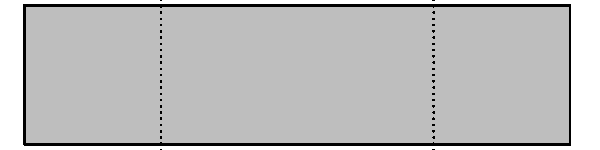
\includegraphics[width=0.20\linewidth, height=0.05\linewidth]{Table_figures/bar7.pdf} &   &   \\ 
  Cetartiodactyla & genus & 100/128 & 
\includegraphics[width=0.20\linewidth, height=0.05\linewidth]{Table_figures/bar8.pdf} & 0.85 & 0.94 \\ 
  \textbf{Cetartiodactyla} & \textbf{species} & \textbf{171/310} & 
\includegraphics[width=0.20\linewidth, height=0.05\linewidth]{Table_figures/bar9.pdf} & \textbf{1.92*} & \textbf{-0.46} \\ 
  Chiroptera & family & 15/18 & 
\includegraphics[width=0.20\linewidth, height=0.05\linewidth]{Table_figures/bar10.pdf} & -0.28 & 0.56 \\ 
  \textbf{Chiroptera} & \textbf{genus} & \textbf{93/202} & 
\includegraphics[width=0.20\linewidth, height=0.05\linewidth]{Table_figures/bar11.pdf} & \textbf{13.47**} & \textbf{1.1} \\ 
  \textbf{Chiroptera} & \textbf{species} & \textbf{215/1053} & 
\includegraphics[width=0.20\linewidth, height=0.05\linewidth]{Table_figures/bar12.pdf} & \textbf{8.82**} & \textbf{1.22} \\ 
  Cingulata & family & 1/1 & 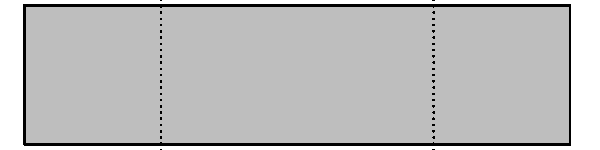
\includegraphics[width=0.20\linewidth, height=0.05\linewidth]{Table_figures/bar13.pdf} &   &   \\ 
  Cingulata & genus & 8/9 & 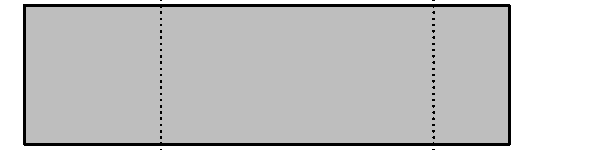
\includegraphics[width=0.20\linewidth, height=0.05\linewidth]{Table_figures/bar14.pdf} & 1.51 & -1.57 \\ 
  \textbf{Cingulata} & \textbf{species} & \textbf{9/29} & 
\includegraphics[width=0.20\linewidth, height=0.05\linewidth]{Table_figures/bar15.pdf} & \textbf{1.9*} & \textbf{0.11} \\ 
  Dasyuromorphia & family & 2/2 & 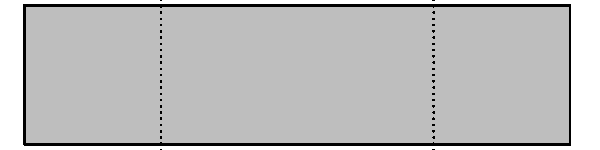
\includegraphics[width=0.20\linewidth, height=0.05\linewidth]{Table_figures/bar16.pdf} &   &   \\ 
  Dasyuromorphia & genus & 8/22 & 
\includegraphics[width=0.20\linewidth, height=0.05\linewidth]{Table_figures/bar17.pdf} & -0.75 & -1.07 \\ 
  Dasyuromorphia & species & 9/64 & 
\includegraphics[width=0.20\linewidth, height=0.05\linewidth]{Table_figures/bar18.pdf} & -0.88 & -0.34 \\ 
  Dermoptera & family & 1/1 & 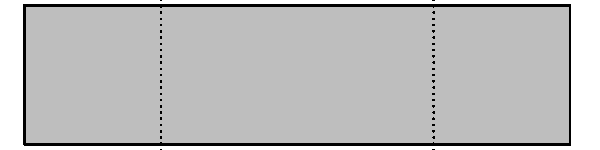
\includegraphics[width=0.20\linewidth, height=0.05\linewidth]{Table_figures/bar19.pdf} &   &   \\ 
  Dermoptera & genus & 1/2 & 
\includegraphics[width=0.20\linewidth, height=0.05\linewidth]{Table_figures/bar20.pdf} &   &   \\ 
  Dermoptera & species & 1/2 & 
\includegraphics[width=0.20\linewidth, height=0.05\linewidth]{Table_figures/bar21.pdf} &   &   \\ 
  Didelphimorphia & family & 1/1 & 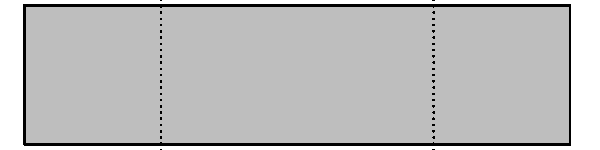
\includegraphics[width=0.20\linewidth, height=0.05\linewidth]{Table_figures/bar22.pdf} &   &   \\ 
  Didelphimorphia & genus & 16/16 & 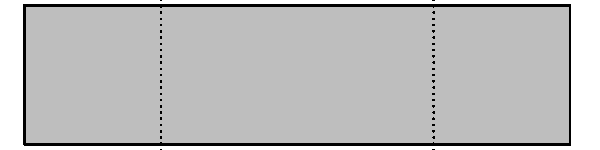
\includegraphics[width=0.20\linewidth, height=0.05\linewidth]{Table_figures/bar23.pdf} &   &   \\ 
  Didelphimorphia & species & 42/84 & 
\includegraphics[width=0.20\linewidth, height=0.05\linewidth]{Table_figures/bar24.pdf} & -1.65 & 0.2 \\ 
  Diprotodontia & family & 11/11 & 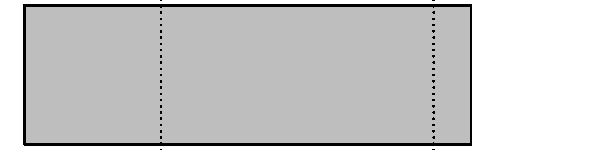
\includegraphics[width=0.20\linewidth, height=0.05\linewidth]{Table_figures/bar25.pdf} &   &   \\ 
  Diprotodontia & genus & 25/38 & 
\includegraphics[width=0.20\linewidth, height=0.05\linewidth]{Table_figures/bar26.pdf} & -1.13 & -1.31 \\ 
  Diprotodontia & species & 31/126 & 
\includegraphics[width=0.20\linewidth, height=0.05\linewidth]{Table_figures/bar27.pdf} & 0.48 & -1.77 \\ 
  Erinaceomorpha & family & 1/1 & 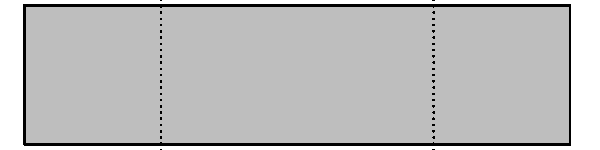
\includegraphics[width=0.20\linewidth, height=0.05\linewidth]{Table_figures/bar28.pdf} &   &   \\ 
  Erinaceomorpha & genus & 10/10 & 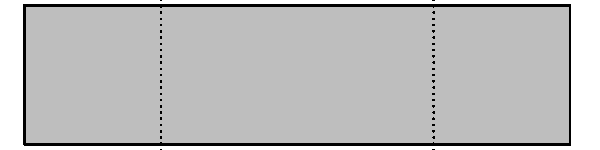
\includegraphics[width=0.20\linewidth, height=0.05\linewidth]{Table_figures/bar29.pdf} &   &   \\ 
  Erinaceomorpha & species & 21/22 & 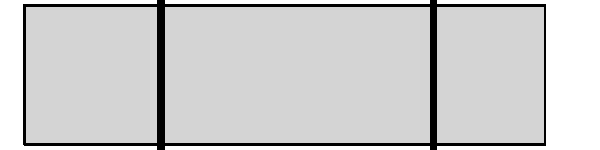
\includegraphics[width=0.20\linewidth, height=0.05\linewidth]{Table_figures/bar30.pdf} & -1.07 & -0.2 \\ 
  Hyracoidea & family & 1/1 & 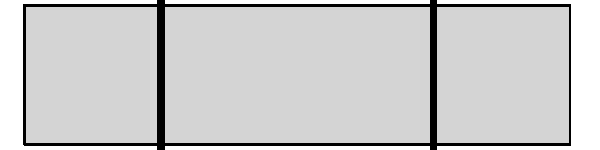
\includegraphics[width=0.20\linewidth, height=0.05\linewidth]{Table_figures/bar31.pdf} &   &   \\ 
  Hyracoidea & genus & 1/3 & 
\includegraphics[width=0.20\linewidth, height=0.05\linewidth]{Table_figures/bar32.pdf} &   &   \\ 
  Hyracoidea & species & 1/4 & 
\includegraphics[width=0.20\linewidth, height=0.05\linewidth]{Table_figures/bar33.pdf} &   &   \\ 
  Lagomorpha & family & 2/2 & 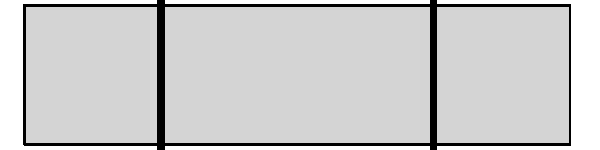
\includegraphics[width=0.20\linewidth, height=0.05\linewidth]{Table_figures/bar34.pdf} &   &   \\ 
  Lagomorpha & genus & 5/12 & 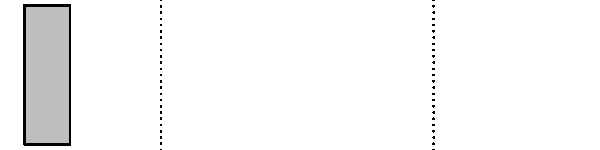
\includegraphics[width=0.20\linewidth, height=0.05\linewidth]{Table_figures/bar35.pdf} & -1.06 & -0.95 \\ 
  Lagomorpha & species & 12/86 & 
\includegraphics[width=0.20\linewidth, height=0.05\linewidth]{Table_figures/bar36.pdf} & -0.62 & -1.88 \\ 
  Macroscelidea & family & 1/1 & 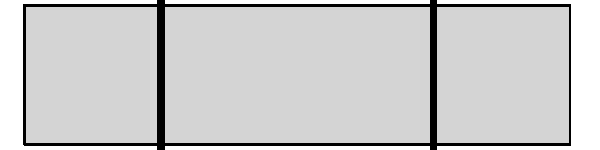
\includegraphics[width=0.20\linewidth, height=0.05\linewidth]{Table_figures/bar37.pdf} &   &   \\ 
  Macroscelidea & genus & 4/4 & 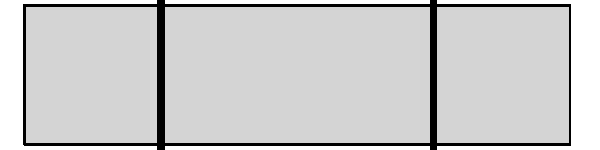
\includegraphics[width=0.20\linewidth, height=0.05\linewidth]{Table_figures/bar38.pdf} &   &   \\ 
  Macroscelidea & species & 12/15 & 
\includegraphics[width=0.20\linewidth, height=0.05\linewidth]{Table_figures/bar39.pdf} & -1.3 & -1.06 \\ 
  Microbiotheria & family & 1/1 & 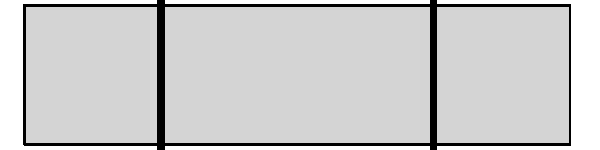
\includegraphics[width=0.20\linewidth, height=0.05\linewidth]{Table_figures/bar40.pdf} &   &   \\ 
  Microbiotheria & genus & 1/1 & 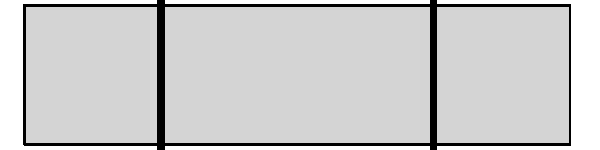
\includegraphics[width=0.20\linewidth, height=0.05\linewidth]{Table_figures/bar41.pdf} &   &   \\ 
  Microbiotheria & species & 1/1 & 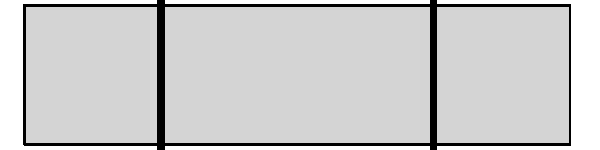
\includegraphics[width=0.20\linewidth, height=0.05\linewidth]{Table_figures/bar42.pdf} &   &   \\ 
  Monotremata & family & 2/2 & 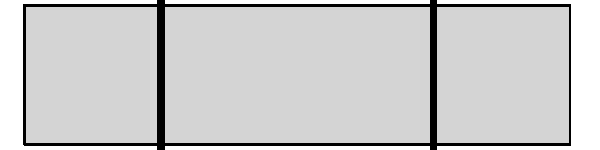
\includegraphics[width=0.20\linewidth, height=0.05\linewidth]{Table_figures/bar43.pdf} &   &   \\ 
  Monotremata & genus & 2/3 & 
\includegraphics[width=0.20\linewidth, height=0.05\linewidth]{Table_figures/bar44.pdf} & -0.72 & -0.69 \\ 
  Monotremata & species & 2/4 & 
\includegraphics[width=0.20\linewidth, height=0.05\linewidth]{Table_figures/bar45.pdf} & -0.97 & -0.97 \\ 
  Notoryctemorphia & family & 1/1 & 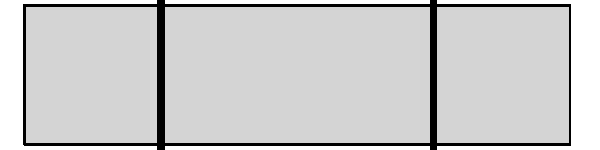
\includegraphics[width=0.20\linewidth, height=0.05\linewidth]{Table_figures/bar46.pdf} &   &   \\ 
  Notoryctemorphia & genus & 1/1 & 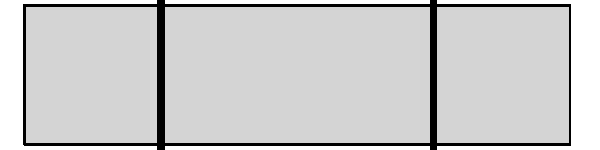
\includegraphics[width=0.20\linewidth, height=0.05\linewidth]{Table_figures/bar47.pdf} &   &   \\ 
  Notoryctemorphia & species & 0/2 & 
\includegraphics[width=0.20\linewidth, height=0.05\linewidth]{Table_figures/bar48.pdf} &   &   \\ 
  Paucituberculata & family & 1/1 & 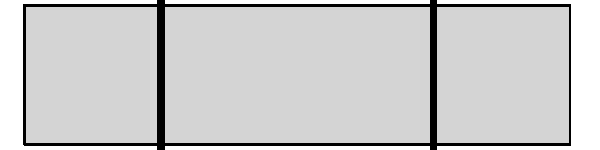
\includegraphics[width=0.20\linewidth, height=0.05\linewidth]{Table_figures/bar49.pdf} &   &   \\ 
  Paucituberculata & genus & 3/3 & 
\includegraphics[width=0.20\linewidth, height=0.05\linewidth]{Table_figures/bar50.pdf} &   &   \\ 
  Paucituberculata & species & 5/5 & \includegraphics[width=0.20\linewidth, height=0.05\linewidth]{Table_figures/bar51.pdf} &   &   \\ 
  Peramelemorphia & family & 2/2 & \includegraphics[width=0.20\linewidth, height=0.05\linewidth]{Table_figures/bar52.pdf} &   &   \\ 
  Peramelemorphia & genus & 7/7 & \includegraphics[width=0.20\linewidth, height=0.05\linewidth]{Table_figures/bar53.pdf} &   &   \\ 
  Peramelemorphia & species & 16/18 & \includegraphics[width=0.20\linewidth, height=0.05\linewidth]{Table_figures/bar54.pdf} & -0.13 & 0.97 \\ 
  Perissodactyla & family & 3/3 & \includegraphics[width=0.20\linewidth, height=0.05\linewidth]{Table_figures/bar55.pdf} &   &   \\ 
  Perissodactyla & genus & 6/6 & \includegraphics[width=0.20\linewidth, height=0.05\linewidth]{Table_figures/bar56.pdf} &   &   \\ 
  Perissodactyla & species & 10/16 & \includegraphics[width=0.20\linewidth, height=0.05\linewidth]{Table_figures/bar57.pdf} & -0.07 & -2.63 \\ 
  Pholidota & family & 1/1 & \includegraphics[width=0.20\linewidth, height=0.05\linewidth]{Table_figures/bar58.pdf} &   &   \\ 
  Pholidota & genus & 1/1 & \includegraphics[width=0.20\linewidth, height=0.05\linewidth]{Table_figures/bar59.pdf} &   &   \\ 
  Pholidota & species & 4/8 & \includegraphics[width=0.20\linewidth, height=0.05\linewidth]{Table_figures/bar60.pdf} & 1.18 & 0.94 \\ 
  Pilosa & family & 4/5 & \includegraphics[width=0.20\linewidth, height=0.05\linewidth]{Table_figures/bar61.pdf} & 1.87 & 2 \\ 
  Pilosa & genus & 4/5 & \includegraphics[width=0.20\linewidth, height=0.05\linewidth]{Table_figures/bar62.pdf} & -0.96 & 0.36 \\ 
  \textbf{Pilosa} & \textbf{species} & \textbf{5/29} & \includegraphics[width=0.20\linewidth, height=0.05\linewidth]{Table_figures/bar63.pdf} & \textbf{1.28} & \textbf{2.38*} \\ 
  Primates & family & 15/15 & \includegraphics[width=0.20\linewidth, height=0.05\linewidth]{Table_figures/bar64.pdf} &   &   \\ 
  Primates & genus & 48/68 & \includegraphics[width=0.20\linewidth, height=0.05\linewidth]{Table_figures/bar65.pdf} & -0.35 & -1.33 \\ 
  Primates & species & 64/351 & \includegraphics[width=0.20\linewidth, height=0.05\linewidth]{Table_figures/bar66.pdf} & -0.67 & -1.27 \\ 
  Proboscidea & family & 1/1 & \includegraphics[width=0.20\linewidth, height=0.05\linewidth]{Table_figures/bar67.pdf} &   &   \\ 
  Proboscidea & genus & 2/2 & \includegraphics[width=0.20\linewidth, height=0.05\linewidth]{Table_figures/bar68.pdf} &   &   \\ 
  Proboscidea & species & 2/3 & \includegraphics[width=0.20\linewidth, height=0.05\linewidth]{Table_figures/bar69.pdf} & -0.69 & -0.69 \\ 
  Rodentia & family & 18/32 & \includegraphics[width=0.20\linewidth, height=0.05\linewidth]{Table_figures/bar70.pdf} & 0.66 & -0.98 \\ 
  Rodentia & genus & 82/450 & \includegraphics[width=0.20\linewidth, height=0.05\linewidth]{Table_figures/bar71.pdf} & -1.66 & 1.55 \\ 
  \textbf{Rodentia} & \textbf{species} & \textbf{90/2094} & \includegraphics[width=0.20\linewidth, height=0.05\linewidth]{Table_figures/bar72.pdf} & \textbf{2.76*} & \textbf{2.34*} \\ 
  Scandentia & family & 2/2 & \includegraphics[width=0.20\linewidth, height=0.05\linewidth]{Table_figures/bar73.pdf} &   &   \\ 
  Scandentia & genus & 2/5 & \includegraphics[width=0.20\linewidth, height=0.05\linewidth]{Table_figures/bar74.pdf} & -0.74 & -0.74 \\ 
  Scandentia & species & 3/20 & \includegraphics[width=0.20\linewidth, height=0.05\linewidth]{Table_figures/bar75.pdf} & -1.88 & -0.84 \\ 
  Sirenia & family & 2/2 & \includegraphics[width=0.20\linewidth, height=0.05\linewidth]{Table_figures/bar76.pdf} &   &   \\ 
  Sirenia & genus & 2/2 & \includegraphics[width=0.20\linewidth, height=0.05\linewidth]{Table_figures/bar77.pdf} &   &   \\ 
  Sirenia & species & 4/4 & \includegraphics[width=0.20\linewidth, height=0.05\linewidth]{Table_figures/bar78.pdf} &   &   \\ 
  Soricomorpha & family & 3/4 & \includegraphics[width=0.20\linewidth, height=0.05\linewidth]{Table_figures/bar79.pdf} & -0.98 & -0.99 \\ 
  \textbf{Soricomorpha} & \textbf{genus} & \textbf{19/43} & \includegraphics[width=0.20\linewidth, height=0.05\linewidth]{Table_figures/bar80.pdf} & \textbf{7.11**} & \textbf{2.59**} \\ 
  \textbf{Soricomorpha} & \textbf{species} & \textbf{21/392} & \includegraphics[width=0.20\linewidth, height=0.05\linewidth]{Table_figures/bar81.pdf} & \textbf{10.65**} & \textbf{3.56**} \\ 
  Tubulidentata & family & 1/1 & \includegraphics[width=0.20\linewidth, height=0.05\linewidth]{Table_figures/bar82.pdf} &   &   \\ 
  Tubulidentata & genus & 1/1 & \includegraphics[width=0.20\linewidth, height=0.05\linewidth]{Table_figures/bar83.pdf} &   &   \\ 
  Tubulidentata & species & 1/1 & \includegraphics[width=0.20\linewidth, height=0.05\linewidth]{Table_figures/bar84.pdf} &   &   \\ 
   \hline
\hline
\label{Table_results}
\end{longtable}

% NC: Can probably cut words from the table legend too 

Among the mammalian orders containing OTUs with no available cladistic data, only six orders had significantly clustered data (Carnivora, Cetartiodactyla, Chiroptera and Soricomorpha at both species- and genus-level and Afrosoricida and Pholidota at the species-level only) and no order had significantly overdispersed data at any taxonomic level (Table~\ref{Table_data_structure}).

Two contrasting results are shown in Figure \ref{Figure_example_coverage} with randomly distributed OTUs with cladistic data in Primates (Figure \ref{Figure_example_coverage}A) and phylogenetically clustered OTUs with cladistic data in Carnivora (mainly Canidae; Figure \ref{Figure_example_coverage}B).

\begin{figure}[!htbp]
\centering
    \includegraphics[width=1\textwidth]{example_coverage.pdf}
\caption{Phylogenetic distribution of species with available cladistic data across two mammalian orders (A: Primates; B: Carnivora).
Edges are colored in grey when no cladistic data is available for a species and in blue when data is available.}
\label{Figure_example_coverage}
\end{figure}

%---------------------------------------------
%
%       DISCUSSION
%
%---------------------------------------------

\section{Discussion}
Our results show that although phylogenetic relationships among living mammals are well-resolved \citep[e.g.][]{FritzTree,meredithimpacts2011,May-Collado-PeerJ} % TG: note that we can reduce the cites here (for the world count in the refs). All three are cited only one time (here). We can save some cites by using \cite{BinindaEmonds,wilson2005mammal} that are cited all along the text already.
% NC: Yep good idea.
, most of the data used to build these phylogenies is molecular, and very little cladistic data is available for living mammals compared to fossil mammals \citep[e.g.][]{O'Leary08022013,ni2013oldest}.
This has implications for building Total Evidence phylogenies containing both living and fossil mammals, as without sufficient cladistic data for living species, fossil placements in these trees are very uncertain \citep{GuillermeCooper}.
Cladistic data coverage in living mammals varies across taxonomic levels and in its phylogenetic distribution.
Higher taxonomic levels are always better sampled than lower ones and within these taxonomic levels, the available data is mostly randomly distributed across the phylogeny, apart from in six orders).

The number of living mammalian taxa with no available cladistic data was surprisingly high at the species-level: only six out of 28 orders have a high coverage of taxa with available cladistic data (and two of the 28 orders are monospecific!).
This high coverage threshold of 75\% of taxa with available cladistic data represents the minimum amount of data required before missing data has a significant effect on the topology of Total Evidence trees \citep{GuillermeCooper}.
Beyond this threshold, there is considerable displacement of wildcard taxa (\textit{sensu} \citep{kearneyfragmentary2002}) and decreases in clade conservation \citep{GuillermeCooper}.
Therefore we expect a high probability of topological artefacts for the placement of fossil taxa at the species-level in most mammalian orders.
However, data coverage seems to be less of an issue at higher taxonomic levels (i.e. genus- and family-level).
This point is important from a practical point of view because of the slight discrepancy between the neontological and palaeontological concept of species.
While neontological species are described using morphology, genetic distance, spatial distribution and even behaviour, palaeontological species can be based only on morphological, spatial and temporal data \citep[e.g.][]{ni2013oldest}.
Because of this, most palaeontological studies are using the genus as their smallest OTU \citep[e.g.][]{ni2013oldest,O'Leary08022013}.
Thus data availability at the genus-level in living mammals should be our primary concern when aiming to build phylogenies of living and fossil taxa.

When only a few species with cladistic data are available, the ideal scenario is for them to be phylogenetically overdispersed (i.e. that there is data for at least every sub-clade) to maximize the possibilities of a fossil branching from the right clade.
The second best scenario is that species with cladistic data are randomly distributed across the phylogeny. 
In this scenario we expect no special bias in the placement of the fossil \citep{GuillermeCooper}, it is therefore encouraging that for most orders, species with cladistic data were randomly distributed across the phylogeny of each order.
The worst case scenario for fossil placement is that species with cladistic data are phylogenetically clustered. 
In this situation we expect two major biases to occur: first, the fossil will not be able to branch within a clade containing no data, and second, the fossil will have a higher probability, at random, of branching within the clade containing most of the available data.
This means that fossils with uncertain phylogenetic affinities (\textit{incertae sedis}) will have a higher probability of branching within the most sampled clade just by chance.
Our results suggest that this may be an issue, at the genus-level, in Carnivora, Cetartiodactyla, Chiroptera and Soricomorpha. 
For example, a Carnivora fossil will be unable to branch in the Herpestidae that has no species with cladistic data, and will also have more chance to branch, randomly, within the Canidae clade than any other clade in Carnivora (Figure \ref{Figure_example_coverage}B).
Thus, in Total Evidence trees, placements of some carnivoran fossils should considered with caution. 
% NC: Trying not to piss off GraHam - really it's weird stuff appearing in Carnivora that we are concerned by, not all Carnivora. TG: I think it's mainly Graham's work that focuses on canids.
In this study, we treated all cladistic matrices as equal in a similar way to molecular matrices. 
For example, if matrix A contained 100 characters for taxa X and Y, and matrix B contained 50 different characters for taxa X and Z, we assumed that both matrices can be combined in a supermatrix containing 150 independent characters for taxon X, 100 for taxon Y and 50 for taxon Z.
Unfortunately, cladistic data cannot always be treated in this way because some characters may overlap.
For example, if matrix A has a character coding for the shape of a particular morphological feature and matrix B has a character coding for the presence of this same morphological feature and a second character coding for its shape, then these three characters are non-independent compound characters \citep{Brazeau2011}.
However, in reasonably sized matrices (\textgreater 100 characters; \citealp{GuillermeCooper,harrisonamong-character2014}) it is more likely that a number of characters are consistently conserved among the different matrices and thus easily combinable.
For example, within the Primate cladistic literature, the character \textit{p7} - the size of the $4^{th}$ lower premolar paraconid - has been used consistently for \textgreater 15 years \citep[e.g.][]{ross1998phylogenetic,marivaux2005anthropoid,kay2008anatomy,boyer2010astragalar,ni2013oldest} and can therefore be combined among the matrices.
A conservative approach to avoid compound characters would be to select only the most recent matrix for each group, but this would result in the loss of a lot of data.

Despite the absence of good cladistic data coverage for living mammals, the Total Evidence methods still seems to be the most promising way of combining living and fossil data for macroevolutionary analyses. 
Following the recommendations in \citep{GuillermeCooper}, we need to code cladistic characters for as many living species possible. 
Fortunately, data for living mammals is usually readily available in natural history collections, therefore, we propose that an increased effort be put into coding morphological characters from living species, possibly by engaging in collaborative data collection projects through web portals such as \textit{Morphobank} \citep{morphobank}.
% NC: Still feels like it needs one final sentence to round it all off. Many something like below, but less crappy:
Such an effort would be valuable not only to phylogeneticists, but also to any researcher focusing understanding macroevolutionary patterns and processes.%interested in the diversity of life on Earth.

%Biology letters various stuff
\section{Ethics statement}
\section{Data accessibility statement}
All data and analysis code is available on GitHub (\url{https://github.com/TGuillerme/Missing_living_mammals}).
\section{Authors' Contributions}
T.G. and N.C conceived and designed the experiments. T.G. performed the experiments and analysed the data. T.G. and N.C. contributed to the writing of the manuscript. All authors approved the final version of the manuscript.
\section{Competing Interests}
We have no competing interests.
\section{Acknowledgements}
David Bapst, Graeme Lloyd, Nick Matzke and April Wright.
\section{Funding statement}
This work was funded by a European Commission CORDIS Seventh Framework Programme (FP7) Marie Curie CIG grant (proposal number: 321696).

\bibliographystyle{sysbio}
\bibliography{References}

%\section{SOM}
\newcommand{\beginsupplement}{%
    \setcounter{table}{0}
    \renewcommand{\thetable}{S\arabic{table}}%
    \setcounter{figure}{0}
    \renewcommand{\thefigure}{S\arabic{figure}}%
}
\beginsupplement

\noindent{\Large \bf Supplementary Material}

\bigskip

\section{Data collection}
1- Data collection: key words, clade (ordinal) metacharacters, Google Search terms, Google Search protocol, Google Search rarefaction curve.

\subsection{Public repositories}
We downloaded available matrices containing fossil and/or living mammal taxa from the three following data bases using the following list of keywords:

\texttt{Mammalia; Monotremata; Marsupialia; Placentalia; Macroscelidea; Afrosoricida; Tubulidentata; Hyracoidea; Proboscidea; Sirenia; Pilosa; Cingulata; Scandentia; Dermoptera; Primates; Lagomorpha; Rodentia; Erinaceomorpha; Soricomorpha; Cetacea; Artiodactyla; Cetartiodactyla; Chiroptera; Perissodactyla; Pholidota; Carnivora; Didelphimorphia; Paucituberculata; Microbiotheria; Dasyuromorphia; Peramelemorphia; Notoryctemorphia; Diprotodontia}.

Details about each public repository specific search option is listed below. Note that some matrices have been downloaded from more than one database but that it is not an issue since we are interested in the total number of living OTUs and that if some where present in more than one matrix, they still only counted as a unique OTU.

\subsubsection{Morphobank}
We accessed the Morphobank repository (\texttt{http://www.morphobank.org/}) on the 5th of December 2014 and used the keywords listed above in the search menue. We downloaded the data associated with each project matching with the keyword.

\subsubsection{Graeme Lloyd}
We accessed Graeme Lloyd's website repository (\texttt{http://graemetlloyd.com/}) on the 5th of December 2014 and downloaded all the matrices that were available with a direct download link in the mammal data section of the website (\texttt{http://graemetlloyd.com/matrmamm.html}).

\subsubsection{Ross Mounce}
We accessed Ross Mounce's GitHub repository (\texttt{https://github.com/rossmounce}) on the 2nd of December 2014 and downloaded every 601 matrix. We then ran a shell script to select only the matrices that had any text element that match with one of the search terms. To make the matrix selection more thorough, we ignored the keywords case as well as the latin suffix (\textit{ia}, \textit{ata}, \textit{ea}, and \textit{a}).

\subsection{Google scholars}
To make sure we didn't miss any extra matrix that wasn't available on one of these repository, we ran a Google Scholar search on the 5th of January. We used the following key words:

\texttt{\textit{order} ("morphology" OR "morphological" OR "cladistic") AND characters matrix paleontology phylogeny}

were \textit{order} was replaced by all the keywords listed above. For each 33 keywords, we selected the 20 first papers to match the Google search published since 2010 resulting in 660 papers. Among these papers, not all contained relevant data (discrete morphological characters AND mammalian data). We selected only the 20 first results per search term to avoid downloading articles that were to irrelevant. Among the 660 papers, only 50 contained a total of 425 extra living OTUs (figure ~\ref{Supp_figure_google_searches}).
Also we decided to select only the articles published since 2010 because nearly every one of the recent published matrix contains both a fraction of morphological characters and OTUs from previous studies. For example in primates the character \textit{p7} coded first by \cite{ross1998phylogenetic} is reused with the same living species in \cite{seiffert2003fossil}, \cite{marivaux2005anthropoid}, \cite{seiffert2005basal}, \cite{bloch2007new}, \cite{bloch2007new}, \cite{kay2008anatomy}, \cite{silcox2008biogeographic}, \cite{seiffert2009convergent}, \cite{tabuce2009anthropoid}, \cite{boyer2010astragalar}, \cite{seiffert2010fossil}, \cite{marivaux2013djebelemur} and \cite{ni2013oldest}.

\begin{figure}[!htbp]
\centering
    \includegraphics[width=1\textwidth]{Supplementary/Supp_figure_google_searches.pdf}
\caption{Google searches additional OTUs rarefaction curve. The x axis represent the number of google scholar matches (papers, books or abstracts) and the y axis represents the cumulative number of additional living OTUs per google scholar match.}
\label{Supp_figure_google_searches}
\end{figure}

\subsection{Standardising the matrices}
We transformed all the non-nexus matrices (tnt, word, excel, jpeg) to nexus format manually. We then cleaned the nexus matrices by removing any extra information (trees, continuous characters, morphological characters description, molecular data) to end up with nexus matrices containing only the discrete morphological data. We then manually fixed the wrong bionomial names format (e.g. \textit{H. sapiens}) into the correct ones (e.g. \textit{Homo sapiens}) using the abbreviation list in the concerned publications. 

\subsection{Selecting the living OTUs}
Finally we applied a taxonomic matching algorithm to classify the OTUs as either living or fossil. The algorithm is matching every OTU name from every matrix with one of the following taxonomic references: the list of taxa from the Fritz \textit{et al.} supertree (2009) \cite{FritzTree}; the taxonomic list from the Wilson and Reeder's Mammals Species of the World (2005) \cite{wilson2005mammal} and the list of all the mammal fossil from the Paleobio Database (\texttt{http://paleobiodb.org/cgi-bin/bridge.pl?a=login}) accessed on the 13th of Janurary 2015. The OTUs that matched with one of the two first references were considered as living OTUs, the OTUs matching with the third reference were considered as fossil OTUs, finally, the OTUs matching with non of the references were discarded (figure ~\ref{Supp_figure_Taxonomic_algorithm}).

\begin{figure}[!htbp]
\centering
    \includegraphics[width=1\textwidth]{Supplementary/Supp_figure_Taxonomic_algorithm.pdf}
\caption{Taxonomic matching algorithm used in this study. For each matrix, each operational taxonomic units (OTU) is matched with the super tree from Fritz 2009. If the OTU matches, then it is classified as living. Else it is matched with the Wilson \& Reeders 2005 taxonomy list. If the OTU matches, then it is classified as living. Else it is matched with the Paleo Database list of mammals. If the OTU matches, then it is classified as fossil. Else it is ignored.}
\label{Supp_figure_Taxonomic_algorithm}
\end{figure}

\bibliographystyle{vancouver}
\bibliography{Supp_References}


\section{Data structure}
%Tables
%Figures

\section{Supplementary results}



%END
\end{document}
